% https://home.hirosaki-u.ac.jp/masumi/100/
\documentclass[a4paper,12pt]{jsreport}
\usepackage{bm}
\usepackage[dvipdfmx]{graphicx}
\usepackage{ascmac}

\title{卒論・修論を\LaTeX で書く}
\author{弘前大学理工学部地球環境防災学科\\
学籍番号 名前}
\date{2020年吉日}

\begin{document}
\maketitle
\tableofcontents

\chapter{はじめに}

最初はイントロ的なことを書く。
\section{現状と問題点}

最近の現状と問題点とか。

\section{解決策の提案}

こうしたらいい,とか。

\section{数式の書き方}

アインシュタイン方程式は以下の通りである。
\begin{equation}
    R_{\mu\nu} - \frac{1}{2} g_{\mu\nu} R = 
    \frac{8\pi G}{c^2} T_{\mu\nu}
\end{equation}



\chapter{つぎに}

この辺から本番。

\section{文献の引用の仕方} 

データは参考文献\cite{rika} にあったものを使った.
この文献\cite{ten}も参考にした。

\section{図の挿入の仕方}
\begin{figure}[h]
  \begin{center}
    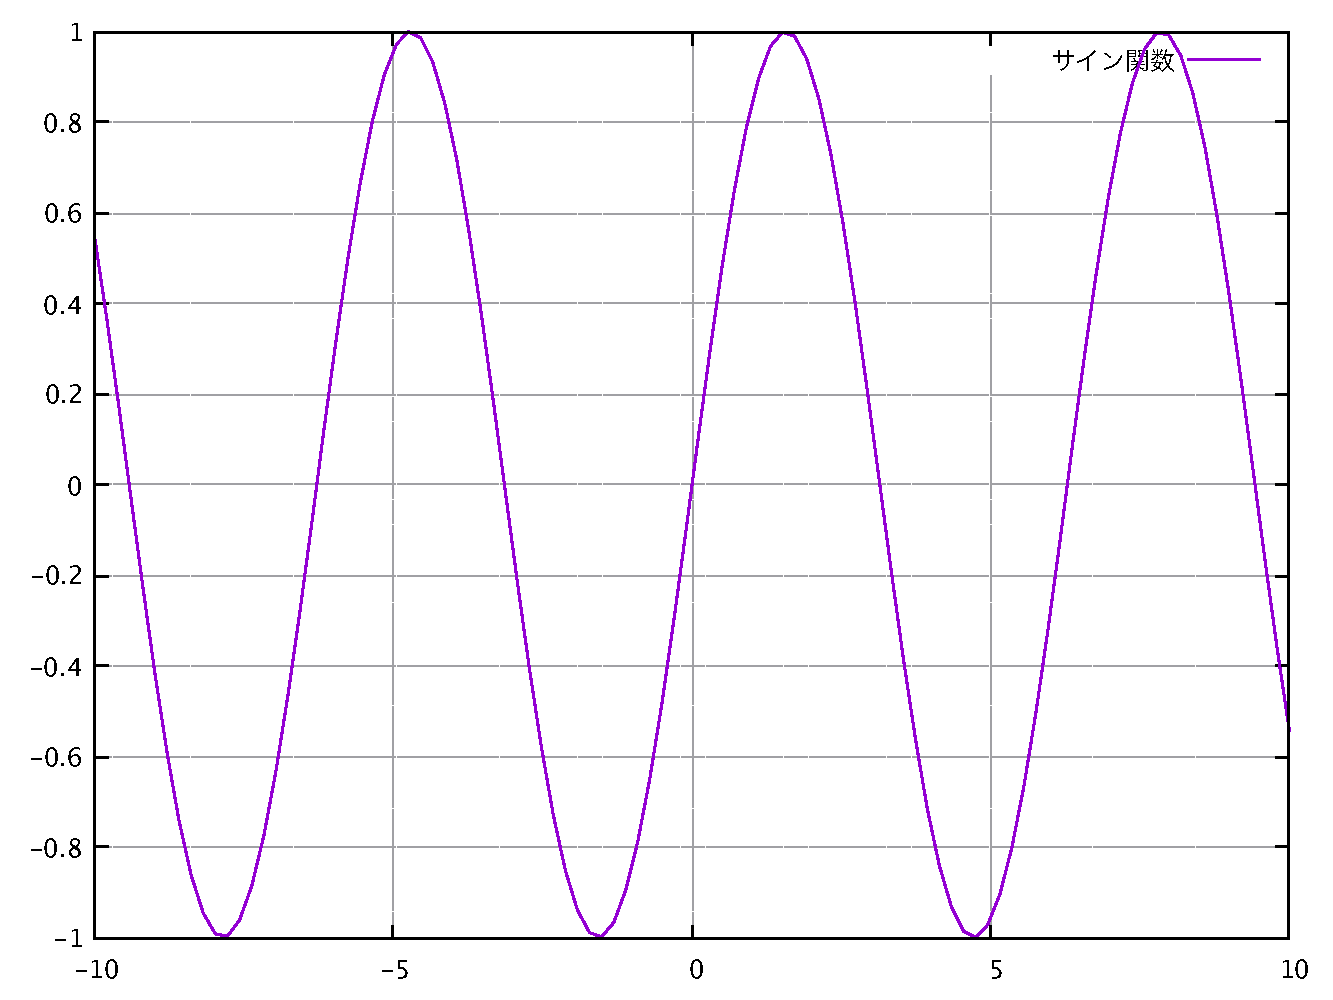
\includegraphics[width=7cm]{./plot1.pdf}
    \caption{サイン関数のグラフ}
  \end{center}
\end{figure}


\chapter{最後に}

結論とか,まとめとか。
最後にいうのもなんだが,ベクトルの書き方。
\begin{itemize}
  \item 普通の$\alpha$は\verb|\alpha|で書く。
  \item \verb|$\vec{\alpha}$| で $\vec{\alpha}$
  \item \verb|\usepackage{bm}| している場合は
        \verb|$\bm{\alpha}$| で $\bm{\alpha}$
  \item 並べると,$\alpha$, $\vec{\alpha}$, $\bm{\alpha}$
\end{itemize}


\chapter*{謝辞}

謝辞には第何章とかの番号をつけなくてもよいので,そんなときは,
\verb|\chapter*{ }| という具合に書きます。

みなさん,ありがとう.(普通の人が見るのは,イントロと謝辞だけ... 
という説もあるから,忘れないで書く.)

\appendix
\chapter{付録があるときは}
プログラム文とかを書いてページ数を稼ぎたいときは,
以下のようにしてみます。

\begin{verbatim}
#include <iostream>
using namespace std;
int main() {  
    for(int i = 1; i <= 5; i++) {
        cout << "こんにちは, C++ の世界!   "  << i << endl;
    }
    return 0;
}
\end{verbatim}
\verb|\usepackage{ascmac}|して\verb|screen| 環境を使うと,枠がつきます。
\begin{screen}
\begin{verbatim}
#include <iostream>
using namespace std;
int main() {  
    for(int i = 1; i <= 5; i++) {
        cout << "こんにちは, C++ の世界!   "  << i << endl;
    }
    return 0;
}
\end{verbatim}
\end{screen}

\begin{thebibliography}{99}
\bibitem{rika} 国立天文台編,理科年表 (丸善)
\bibitem{ten} 天文年鑑,誠文堂新光社。
\end{thebibliography}

\end{document}
